\documentclass[12pt,titlepage,a4paper]{article}


\usepackage{amsthm}
\usepackage{amsmath,empheq}
\usepackage{xltxtra}
\usepackage{amssymb}
\usepackage{graphicx}
\usepackage{unicode-math}
\usepackage{framed}
\usepackage[top=1in, bottom=1in, left=0.5in, right=0.5in]{geometry}
\usepackage{tabularx}
\usepackage{longtable}
\usepackage{ragged2e}
\usepackage{indentfirst}
\usepackage[algoruled]{algorithm2e}
\usepackage[keys]{cryptocode}
\usepackage{float}
\usepackage{hyperref}
\usepackage{tikz}


\usetikzlibrary{arrows}


\hypersetup{
    colorlinks,
    citecolor=black,
    filecolor=black,
    linkcolor=black,
    urlcolor=black
}

\newcommand{\HRule}{\rule{\linewidth}{0.5mm}}

\setmainfont{CMU Serif}

\author{Andrikopoulos Konstantinos\\
Dimitris Kolotouros}
\date{\today}
\title{mpOTR protocol specification}

\setcounter{secnumdepth}{6}

\begin{document}

%Define the myinput macro for algorithm2e
\newlength\mylen
\newcommand\KwExtraIn[1]{%
	\settowidth\mylen{\KwIn{}}%
	\setlength\hangindent{\mylen}%
	\hspace*{\mylen}#1\\}

\newcommand\NextYear{%
  \advance\year by 1 \the\year\advance\year by -1}
\newcommand\PrevYear{%
  \advance\year by -1 \the\year\advance\year by 1}

\begin{titlepage}
\centering

% Upper part of the page

\includegraphics{Pyrforos.png}\\[1cm]
%\textsc{\LARGE Σχολή \\ Ηλεκτρολόγων Μηχανικών \\[-3pt] και \\[6pt] Μηχανικών Υπολογιστών}


% Branch

\vspace{1cm}

% Title
\HRule \\[0.4cm]

{\huge \bfseries Multiparty Off-The-Record chat protocol\\} %\\

\vspace{0.4cm}
\HRule \\[0.4cm]

%Subtitle
{\Large Protocol specification}


% Authors
\vfill
\begin{center}
\large
%Add authors one after another with the same format
%\begin{framed}
Andrikopoulos Konstantinos\\
Kolotouros Dimitrios

%\end{framed}


\vfill
\the\year\

\end{center}



\end{titlepage}
\tableofcontents
\newpage
{
\section{Overview}
The goal of our project is to implement a library for private group conversations.
This library is implemented as part of the Off-The-Record (OTR) library (libotr), which only offered private conversations between two participants.
Our work is heavily based on the mpotr paper \cite{mpotr}.
Following the OTR conventions, the term "private" is used to describe the properties of casual real-life conversations:

\begin{itemize}
  \item confidentiality
  \item authentication
  \item repudiation
  \item forward secrecy.
\end{itemize}

In order to implement the mpOTR protocol described in \cite{mpotr}, we had to specify the subprotocols that were treated as black boxes and not fully described.
We propose a Deniable Signature Key Exchange (DSKE) based on the pairwise triple Diffie-Hellman protocol CITE TRIPLE DH HERE.
For a Group Key Agreement (GKA) we use the protocol proposed in \cite{mpenc} but using classic Diffie-Hellman (ie not ECDH).

We also propose an improvement in the shutdown phase originally suggested in \cite{mpotr},
utilising a relatively new cryptographic primitive called "cryptographic accumulator".

\section{Threat Model}
\label{threat_model}
In \cite{mpotr} a threat model was specified. Specifically, three adversaries are introduced.

\subsection{Security adversary $\mathcal{O}$}
This adversary's goal is to read the messages of the chatroom.
Let $T_c^{\hat{X}}$ be the transcript of chatroom $c$ owned by participant $\hat{X}$.
Then, $\mathcal{O}$ is successful, if he can read any message from transcript $T_c^{\hat{A}}$, where $\hat{A}$ is an honest participant, without receiving it from transcript $T_c^{\hat{X}}$ for any participant $\hat{X}$ where $\hat{X} \ne \hat{A}$.
While $\mathcal{O}$ can, both passively and actively, control the network, decrypt messages sent in other chatrooms and even participate in other sessions, he has limited access on the room he wants to attack.
Not only can he not participate in the session under attack, but he also cannot ask for any secret shared between the participants of the specific room.
He has the ability to inject messages of his liking in the chatroom by asking an, otherwise honest, user.
In essence $\mathcal{O}$ is a somewhat formal definition of the notion of IND-CPA attacks in the multiparty setting.

\subsection{Privacy adversary $\mathcal{M}$}
The privacy adversary aims to break the deniability of the protocol.
He is successful if he can prove to a judge $\mathcal{J}$ that a user $\hat{A}$ participated in, read messages from or authored messages in chatroom $c$.
His restrictions are very few.
He can collaborate with $\mathcal{J}$ before the creation of $c$, participate fully in $c$ and even force $\hat{A}$ to reveal his long term secrets in front of the judge.

\subsection{Consensus adversary $\mathcal{T}$}
\subsubsection{Definition of Consensus}
For two participants $\hat{A}$ and $\hat{B}$, consensus is reached on $T_{C_1}^{\hat{A}}$ when $\hat{A}$ believes $\hat{B}$ claims to have a transcript $T_{C_2}^{\hat{B}}$ such that:

\vbox{%
\begin{itemize}
  \label{consensus_def}
  \item $C_1$ has the same set of participants as $C_2$;
  \item $C_1$ and $C_2$ are the same chat room instance;
  \item $T_{C_2}^{\hat{B}}$ has the same collection of messages as $T_{C_1}^{\hat{A}}$;
  \item $T_{C_2}^{\hat{B}}$ and $T_{C_1}^{\hat{A}}$  agree an each message's origin.
\end{itemize}
}

Notice that the above definition is not symmetric.
This means that $\hat{A}$ can reach consensus with $\hat{B}$ without necessarily $\hat{B}$ reaching consensus with $\hat{A}$.

The interpretation of the term "collection of messages" is intentionally left unclear.
This way, each application can handle the ordering of the messages in different ways.

\subsubsection{$\mathcal{T}$'s goal}
$\mathcal{T}$ is successful when he is able to force an honest user $\hat{A}$ to believe that consensus is reached with another honest user $\hat{B}$ when at least one condition from \ref{consensus_def} does not hold.
Notice that only $\hat{A}$ and $\hat{B}$ must be honest.
$\mathcal{T}$ can otherwise control other users as he sees fit.

\section{Setup}
\subsection{Offer}
\label{Offer}
During the first phase of the setup procedure, which we call "Offer", the participants calculate a unique session id called $sid_i$. This is a value that will be used to distinguish the current session between other sessions created by the same set of participants. \\

Each participant $\hat{X}$ chooses a random 256-bit value $x_{\hat{X}}$, which is his contribution to the $sid_i$. We define $sid_i$ as the SHA-512 hash of the serialized ordered list that contains every participant's contribution. \\

Each offer message contains the sender's contribution along with his position in the participants list. \\

The participant who wants to initiate the mpOTR protocol, broadcasts an offer message. Once a participant receives an offer message:

\begin{itemize}
	\item[]He checks if the sender's position contained in the message matches his actual position, if not, he rejects the message.

	\item[]He checks if he has already received an offer message from the sender, if so, he rejects the message.

	\item[]He checks if he has already broadcast his own offer message. If not, creates and broadcasts his own offer message.

	\item[]He checks if he has received every participant's contribution. If so, he calculates the $sid_i$ and proceeds to the next setup phase.
\end{itemize}

Notice that these messages are not authenticated and hence the session id must
be verified \emph{after} the participants have exchanged signing keys.


\subsection{Deniable Signature Key Exchange (DSKE)}
\label{DSKE}
In \cite{mpotr} a construction for a DSKE is proposed. Given a deniable
Authenticated Key Exchange\\ (denAKE), two participants of the chat can
generate a deniable and authenticated shared secret. With that secret
they can exchange their ephemeral signing public key in an encrypted and
authenticated fashion, using symmetric algorithms.\\

This is done for every pair of participants. After that, they will all have
created an association table, which associates each participant with their
signing key. Afterwards, the participants must make sure that they all have
constructed the same association table. This is done by each participant
transmitting the hash of the association table (which is sorted in
lexicographical order according to each participant's username). The hash
is signed by the ephemeral signing key. \\

Each participant must verify the signatures in each hash received and also
make sure that each hash is the same with the one he has calculated. If everything
checks out, then he is assured that the association table is the same.

\subsubsection{denAKE}


In \cite{mpotr} no denAKE is specified. We propose the following protocol:

\begin{itemize}

	\item[] Each participant generates a private/public Diffie-Hellman keypair $(A_i, g^{A_i})$, which will be used as a longterm key to idenitfy him to other participants. This
is done only once, when a member first used the protocol, then the key remains
the same for subsequent runs of the protocol.

	\item[] To initiate a denAKE, each participant creates an ephemeral Diffie-Hellman keypair
		$(a_i,g^{a_i})$ used only in this run of the protocol (he uses however the same ephemeral key
		to communicate with all the participants).

	\item[] Then he broadcasts the public components of the longterm and ephemeral keys to
		all chat participants in the tuple $(g^{A_i}, g^{a_i})$. We shall call this
		message a "Handshake Message".

	\item[] When participant $i$ has received a handshake Message $(g^{A_j}, g^{a_j})$ from some
		other participant $j$, she can compute the shared secret, as specified by the triple
		Diffie-Hellman protocol. This secret is $g^{a_ia_j} || g^{A_ia_j} || g^{A_ja_i}$
		.

	\item[] After computing the shared secret she encrypts and mac's a magic number and sends it
		to the other party. This is done to verify that the other party has indeed generated
		the same shared secret and is not an adversary trying to break the forward secrecy
		property of triple Diffie-Hellman, see \ref{confirm_message_explain}. We shall call
		this message a "Confirm Message".

	\item[] When she herself has received the corresponding Confirm Message she is assured that
		the shared secret can be safely used and there is no foul play. Now she
		encrypts-then-macs her signing public key and sends it to the other party. This
		message is called a "Key Message"


	\item[] When a key message is received he first verifies the message using the same mac.
		If the tag checks out he decrypts the key and adds it in the association table.
\end{itemize}

In figure \ref{den_ake_schematic} a schematic description of the protocol is provided.

\paragraph{Order of the concatenation}
When the shared secret is calculated, three values must be concatenated. Since
concatenation is not commutative the two parties must agree on the order that the
concatenation happens.

This is achieved by compare the values $g^{A_i}$ and $g^{A_j}$. If
$g^{A_i} \le g^{A_j}$ then the shared secret is $g^{a_ia_j} || g^{A_ia_j} || g^{A_ja_i}$
If not then the shared secret is $g^{a_ia_j} || g^{A_ja_i} || g^{A_ia_j}$. That is, the
value that is generated using the highest public key takes precedence during the
concatenation.

In the overview of the algorithm above, it was silently assumed that
$g^{A_i} \le g^{A_j}$.

\paragraph{The need of a confirmation message}
\label{confirm_message_explain}
A confirmation message is needed if want to have forward secrecy in this exchange.
We must make sure that we are really speaking with the intended participant. Consider
the following scenario.

An adversary, Eve, creates an ephemeral keypair $(b, g^b)$. Then he poses as Bob to Alice,
and broadcasts a handshake message containing $(g^B,g^b)$ where $g^B$ is Bob's
public longterm key.

After Alice receives the handshake message she can construct the shared secret. Eve
however cannot construct the secret since she does not know Bob's longterm
private key. If Alice starts sending data before confirming that the other party
has indeed arrived at the same secret she is under the danger to lose the forward
secrecy property for all messages she sends with the secret.

Indeed the only reason Eve can't construct the secret that Alice calculated, is
that she doesn't have Bob's longterm private key. This of course means that if
she somehow gets a hold of this key, she can decrypt some messages. This situation
of course does not satisfy the forward secrecy property.


\subsubsection{Properties}

Triple Diffie-Hellman is a protocol that is a) authenticated b) forward secret
and c) deniable.

It is authenticated, because the shared secret can only be calculated by someone
only if he posses one of the longterm private keys (and the corresponding ephemeral
of course).

It is forward secret, because once the ephemeral key has been destroyed, it is
impossible to reconstruct the shared secret even when the longterm
private key is compromised.

It is deniable, because the only values that are exchanged during a protocol run
are the two public keys that a participant will use. Nothing is signed, which means
that nothing can be used to prove that someone took part in a conversation.\\[0.5cm]

Another property of this protocol that comes for free is its very fast key generation
as, basically, any random number can be used as a secret key.

Thus Triple Diffie-Hellman satisfies the properties required in \cite{mpotr} and
can be used as a denAKE.

\begin{figure}[t]
  \fbox{%
    \pseudocode{%
      \textbf{Alice} \< \< \textbf{Bob} \\[][\hline]
      \text{ Choose a random number $x \in Z_p^*$ }\< \< \\
      \< \sendmessageright*{Send \ \left(g^x,g^X\right)} \< \\
      \< \< \text{ Choose a random number $y \in Z_p^*$ } \\
      \< \< s = g^{xy} || g^{Xy} || g^{Yx} \\
      \< \< k_1 = KDF_1(s) \\
      \< \< k_2=KDF_2(s) \\
      \< \sendmessageleft*{Send \ \left(g^y,g^Y\right)} \< \\
      s = g^{xy} || g^{Xy} || g^{Yx} \< \< \\
      k_1 = KDF_1(s) \< \< \\
      k_2 = KDF_2(s) \< \< \\
      \< \sendmessageright*{ Send \\ c = AES_{k_1}("confirm") \\ MAC_{k_2}(c)\ } \< \\
      \< \< \text{Verify mac} \\
      \< \< m = AES^{-1}_{k_1}(c) \\
      \< \< \text{Verify m = "confirm"} \\
      \< \sendmessageleft*{ Send \\ c = AES_{k_1}("confirm") \\ MAC_{k_2}(c)\ } \< \\
      \text{Verify mac} \< \< \\
      m = AES^{-1}_{k_1}(c) \< \< \\
      \text{Verify m = "confirm"} \\
      \< \sendmessageright*{Send \\ c = AES_{k_1}(\pk_a) \\ MAC_{k_2}(c) } \< \\
      \< \< \text{Verify mac} \\
      \< \< \text{Add $\pk_a$ to association table} \\
      \< \sendmessageleft*{Send \\ c = AES_{k_1}(\pk_b) \\ MAC_{k_2}(c) } \< \\
      \text{Verify mac} \< \<  \\
      \text{Add $\pk_b$ to association table} \< \< \\
    }
  }
  \caption{The denAKE protocol, where $X$ and $Y$ are the private parts of the long term keys}
  \label{den_ake_schematic}
\end{figure}

\clearpage
\subsection{GKA}

During this phase the participants derive a shared secret key $g_k$ to be used
as a symmetric encryption key.

The main idea is to compute a combined Diffie-Hellman-like key for all
participants, which will then be used for encryption.

To do this. each participant in the chatroom generates a private exponent.
The shared base is then raised to this exponent. The key agreement begins
by the initiating participant sending his public key to the next participant.

In each step that follows, the participant who just received a list of intermediate
keys from the previous participant must calculate the next intermediate key list and
forward it to the next participant, until the final participant. These messages
shall be called "Upflow Messages".

During the $i$-th iteration, the corresponding participant receives keys from the
$(i - 1)$th participant. and then sends information to the $(i + 1)$th participant.
When the last participant has received the required information, he computes a)the
shared secret and b) the final intermediate key list and then forwards it back to
all previous participants. This message, containing the last intermediate key list
shall be called "Downflow Message".

The other participants now can also caclulate the shared secret and use it for
encryption, using the intermediate key list.

\subsubsection{Detailed description}
For a more detailed description of the protocol we refer to \cite{mpenc}, however
a pseudocode is provided.\\

Algorithm \ref{upflow_algo} presents an overview of how each upflow message is constructed, using the data received from the previous upflow message.\\

Algorithm \ref{downflow_algo} presents an overview of how the final, downflow message is constructed using the data received from the last upflow message.\\


In algorithm \ref{gka_proto_algo} the two previous algorithms (\ref{upflow_algo} and \ref{downflow_algo}) are used in order to execute a complete run of the gka protocol.\\

\begin{algorithm}[H]
	\KwIn{P : participants list}
	\KwExtraIn {InterKeys : previous intermediate key list}
	\KwExtraIn {X : user's secret key}
	\KwExtraIn {N : next participant}
	\KwResult{Sends the new intermediate key list to the next participant}
	\Begin{
	inter\_key\_list := empty\_list

	inter\_key\_list.append( InterKeys.last\_elem() )

	\ForEach{k in InterKeys}
	{
		inter\_key\_list.append( $k^X$ )
	}

	send( N , P || inter\_key\_list)
	}
	\caption{Upflow Message send algorithm}
	\label{upflow_algo}
\end{algorithm}

\vfill
\begin{algorithm}[H]
	\KwIn{P : participants list}
	\KwExtraIn {InterKeys : previous intermediate key list}
	\KwExtraIn {X : user's secret key}
	\KwExtraIn {N : next participant}
	\KwResult{Sends the downflow intermediate key list to the other participants}
	\Begin{
	inter\_key\_list := empty\_list

	\ForEach{k in InterKeys}
	{
		inter\_key\_list.append( $k^X$ )
	}

	inter\_key\_list.reverse()

	send( N , P || inter\_key\_list)
	}
	\caption{Downflow Message send algorithm}
	\label{downflow_algo}
\end{algorithm}

\begin{algorithm}[H]
	\KwIn{P : participants list}
	\KwOut{The shared secret}
	\KwResult{Executes a GKA and produces the shared secret}
	\Begin{

	prev := get\_previous\_participant()

	next := get\_next\_participant()

	x := gka\_genkey()

	\If{prev == NULL}{
		send\_upflow(P, [G], x, next)
		}
	\Else{
			m = receive\_from(prev)

			\If{ m not valid}{
					return error
			}
			\If{ next != NULL}{
				send\_upflow(P, m.key\_list, x, next)
			}
			\Else{
				final\_key := m.key\_list.last\_elem()

				s := $final\_key^x$

				send\_downflow(P, m.key\_list, x)

				return s
			}
	}

	m = wait\_for\_downflow()

	\If{m not valid}{
		return error
	}

	final\_key := m.key\_list[pos]

	s := $final\_key^x$

	return s

	}
	\caption{The GKA protocol}
	\label{gka_proto_algo}
\end{algorithm}

\begin{figure}[H]
  \begin{minipage}{0.49\textwidth}
    \begin{tikzpicture}[scale=.9]
      \def \n {5}
      \def \ndec {4}
      \def \radius {3cm}
      \def \margin {8} % margin in angles, depends on the radius

      \foreach \s in {1,...,\ndec}
      {
        \node[draw, circle] at ({180 + (360/\n * (\s - 1))}:\radius) {$\s$};
        \draw[->, >=latex] ({145 + 36 + (360/\n * (\s - 1))+\margin}:\radius)
          arc ({145 + 36 + (360/\n * (\s - 1))+\margin}:{145 + 36 + 360/\n * (\s)-\margin}:\radius);
      }
      \node[draw, circle] at ({181 + 360/\n * (\n - 1)}:\radius) {$\n$};
    \end{tikzpicture}
    \caption{This diagram demonstrates the upflow of the intermediate keys}
  \end{minipage}
  \begin{minipage}{0.49\textwidth}
    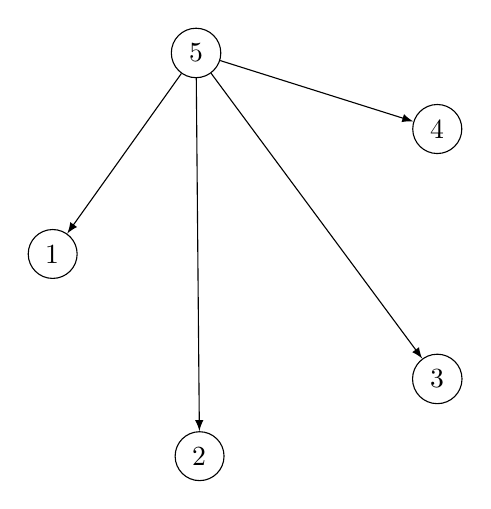
\begin{tikzpicture}[scale=.9]
      \def \n {5}
      \def \ndec {4}
      \def \radius {3cm}
      \def \margin {8} % margin in angles, depends on the radius

      \foreach \s in {1,...,\ndec}
      {
        \node[draw, circle](\s) at ({180 + (360/\n * (\s - 1))}:\radius) {$\s$};
      }
      \node[draw, circle](5) at ({181 + 360/\n * (\n - 1)}:\radius) {$\n$};
      \draw[->, >=latex] (5) -- (1);
      \draw[->, >=latex] (5) -- (2);
      \draw[->, >=latex] (5) -- (3);
      \draw[->, >=latex] (5) -- (4);
    \end{tikzpicture}
    \caption{This diagram demonstrates the downflow of the intermediate keys}
  \end{minipage}
\end{figure}
\subsection{Attest}

During this phase the participants must verify that they agree on the $sid_i$,
and the association table as we mentioned in \ref{Offer} and \ref{DSKE}.
This is needed for two reasons. First because the session id is required before a signing key association table is constructed, and therefore the messages exchanged for the session id calculation can not be signed.
Second because the participants need to verify that they all have the same view of the association table.\\

Each participant calculates the SHA-512 hash of the serialized association table and broadcasts an encrypted and authenticated message that contains both the $sid$ and the calculated hash.
To authenticate the message, the sender uses the ephemeral signing key he has now exchanged with the other participants.
When each participant has received the attest messages from every other participant he must check two things.
He must verify that the hashes of the serialized association table he has received from the other participants are the same with the hash he computed himself.
He also must check that all participants have sent their messages using the same session id.\\

Provided that SHA-512 is a cryptographic hash function an attacker cannot find two signing keys association tables with the same hash.
This means that he is not able to make two participants believe that they have arrived at the same table when they have not.
Also by signing the message with the specific session id, a user implicitly verifies that he is using that particular id for this session.

\section{Communication}

During the communication phase, the participants can exchange authenticated
and encrypted messages using the association table derived from DSKE and the
symmetric encryption key $g_k$ derived from GKA.

\subsection{Origin Authentication}

For origin Authentication we will use public key encryption methods. This is
done because use of symmetric algorithms would require a participant who
wishes to send a message to mac the message $n-1$ times, where $n$ is the
number of the participants.

\subsubsection{Algorithm}

While describing the DSKE we mentioned that an ephemeral signing key is transmitted
by each participant to every other, to be used for message origin verification.

For this purpose we make use of the EdDSA algorithm. This algorithm was selected
for its fast key generation, since a new keypair must be generated in each protocol
run, and its relatively small signature size.

\subsubsection{Signing} \label{signing}

The signature generation is the last step taken before sending a message. This
way we can sign all the properties of the message to be sent, like the $sid$ or the
recipient (if any). We also avoid any manifestations of the Cryptographic Doom
Principle, which states that if a protocol tries to perform \emph{any}
cryptographic operation before verifying the signature or mac on a received
message, it will somehow fail catastrophically and lead to doom.

Symmetrically the signature verification is the first thing that happens before
any other operation is performed on the received message (cryptographic or not).

\subsection{Encryption}

For encryption a shared secret key is used by all the members. This is not a
problem since the origin authentication is provided by the signatures, and
we obviously don't mind any chat member to read a message or we wouldn't
participate in the chat in the first place. For the actual encryption we
use AES-128 in CTR mode.

The use of the CTR mode however has a small pitfall. We must not let the same
nonce be used twice. This is very difficult to achieve in a distributed setting
like a multi-party chat protocol. Despite this we can solve the problem quite
easily. We maintain our original idea of a shared master key, but we don't use
it directly for encryption. Each participant uses the master key and his id in
the chatroom, in order to compute his "personal" encryption key. This encryption
key for participant $p$ is derived as follows:

\[
    K_e = H(ID_p || Key_m)
\]

Provided that $H$ is a cryptographic hash function, an adversary cannot recover
the value $K$ used for encryption as long as he doesn't know the master key.
}

\subsection{Transcript}

In order to execute the shutdown protocol we need to store the transcript of the chatroom.
In reality a seperate transcript is held for the messages from each participant.
The shutdown protocol will then combine all the different transcripts to determine if consensus has been reached.

The transcript is implemented as a linked list. The list is kept sorted in lexicographic order.
When a message is to be added in a transcript list, the list is searched linearly to find the position the new message should be placed.

When user $A$ sends a message he adds that message to the transcript corresponding to himself.
When he receives a message from user $B$ then he adds that message to the transcript corresponding to user $B$.

\section{Shutdown}

During this phase, the participants end the current session and publish their
ephemeral signing keys, to permit modifying the chat transcript. This adds to
the protocol's deniability property. (Notice though, that the protocol is
deniable without publishing the ephemeral signing keys.)

For a session to be terminated, a "Shutdown Message" is sent.
This message signals to other participants that the shutdown phase should be initiated.
It contains the  hash of all the messages sent by the user sending the "Shutdown Message".
When a user receives a "Shutdown Message", he also sends a "Shutdown Message" containing his own messages hash.
If he has already sent his "Shutdown Message" then he does nothing new.

When one participant has received a "Shutdown Message" from all other participants he can send a "Digest Message".
This message contains a digest of all the messages in the chat-room and is calculated as follows:
\begin{itemize}
  \item[] Sort the participants using their usernames in lexicographic order.
  \item[] For each participant $i$ (in that order) calculate the hash $h_i = H(S_i)$, where $S_i$ is set of all the messages sent by this user (sorted in lexicographic order).
  \item[] Calculate the digest $h = H(h_1 || h_2 \dots || h_N)$, where N is the number of participants.
\end{itemize}

When one participant receives a "Digest Message" from some other participant he checks whether the two of them agree on the chat-room transcript.
He simply compares the digest he computed locally to the one sent by the other participant.
He deduces that consensus is reached only if the two digests are the same.

When one participant has received a "Digest Message" from every other participant he broadcasts an "End Message".
This message signifies that the sender will not user the channel to send any messages anymore.
As a result when a participant receives an "End Message" from all other participants, he is certain that he can release his signing secret key.
Now anyone who intercepts the released key can forge chat-room messages.
However all the participants will no longer accept messages signed with the released secret key, and thus it cannot be used to impersonate its previous owner.

\section{Putting it all together}
Using the subprotocols described above we have this protocol:

\begin{algorithm}[H]
  \KwIn{$\mathcal{P}$ : participants list}
	\KwResult{Executes a run of the mpOTR protocol}
	\Begin{

  $sid$ := Offer($\mathcal{P}$)

  $\mathcal{S}$ := DSKE($sid$, $\mathcal{P}$)

  $\mathcal{K}$ := GKA($sid$, $\mathcal{S}$, $\mathcal{P}$)

  $\mathcal{T}$ := Communication($sid$, $\mathcal{K}$, $\mathcal{S}$, $\mathcal{P}$)

  $c$ := Shutdown($sid$, $\mathcal{T}$, $\mathcal{S}$, $\mathcal{P}$)

  \If{$c$ = "consensus"}{
    \Return{"OK"}
  }
  \Else{
    \Return{"Error"}
  }

	}
	\caption{The mpOTR protocol}
	\label{mpotr_algo}
\end{algorithm}

Where $sid$ is the session id, $\mathcal{S}$ is the signing keys association table, $\mathcal{K}$ is the group shared secret, $\mathcal{T}$ is the transcript of the chatroom and finally $c$ s a boolean value which states if consensus has been reached with all participants.

\subsection{Implementation Notice}

The reader should note that while in \cite{mpotr} a chatroom message consistency
check is specified, it is not yet implemented in our protocol. This is done on
purpose since we are still examining the possible optimization in the proposed
method, which is discussed later in this document.

It must also be made clear that at the moment the protocol does not protect
from message reordering, both from an insider or an outsider to the group.

Thus our protocol is at the time vulnerable both to message reordering and replay
attacks. It is also possible for a participant to send different messages to
different participants.

When the shutdown phase is fully implemented the only possible attack would be
to change the order that the messages appear in.

\section{Message consistency in constant space}

In \cite{mpotr} a straightforward approach is followed. In order to check if
each participant has received the same set of messages all the messages from
each user must be stored, and during the shutdown phase be lexicographically
ordered and hashed. While this achieves our purpose it requires $O(M)$ space
where $M$ is the number of messages.

We believe that the same effect can be achieved in constant space by using
cryptographic accumulators. One can find more about this primitive in \cite{accum_def}.

Since such accumulators are collision free but at the same time quasi-commutative,
they are ideal for our purposes. We can feed the accumulator with the incoming
messages in whichever order they arrive at each participant. The quasi-commutative
property guarantees that if two participants have received the same set of messages
then their accumulators will arrive at the same value in the end.

Thus, we have removed the need to store the messages in order to sort them during
the shutdown phase. We only need to store the value of the accumulator which,
of course, is constant.

\section{Participants ordering}

In many cases, the protocol demands some ordering of the participants. For example, in the Offer step of the Setup phase, the sid contributions should be concatenated in some order before hashing them. Same stands for the public signing keys in the association table, during the Attest step. So we define an ordering rule for the participants, that is used whenever an ordering of elements corresponding to participants is needed. \\

Given that the application provides the mpOTR protocol with a unique name describing each participant, we make the convention that every ordering of the participants list is made lexicographically based on that unique name. We also define the position of the participant, as his position in this order, starting counting from zero (0).

\section{Identity Verification}
The identity of a participant is verified during the DSKE phase.
In order for a participant to be verified the fingerprint of his longterm key must be stored in the known fingerprints file, and be explicitly marked as verified.
In our implementation this file is comma separated and is of the form:

\begin{verbatim}
<account_name>,<protocol>,<buddy_name>,<fingerprint>,<is_verified>
\end{verbatim}

The account name is the "address" of the library user in the form username@host, and is provided by the application.
The protocol is a string that is characteristic of the underlying protocol that the specific account uses.
It is again provided by the application.
The buddy name is the nickname that a user is identified with.
For the time being it is the username part of a users "address".
This implies that the underlying protocol provides addresses which do not change often for a user.
It also means that users from multiple hosts are not allowed or else two users with the same username might conflict.
The above holds for a protocol like jabber for example, but is not the case for protocols like IRC.
As a result our implementation is not fully protocol agnostic at this moment.
Finally the fingerprint is the sha256 hash of the public identity key, and the last field is 1 if the key is verified and 0 otherwise.

This file is read during the plugin start up and initializes the list of all known fingerprints.
When a new chatroom is created, each participant is assigned a list with all known fingerprints used by this participant (from the above list).
When a "Handshake Message" is received the participants known fingerprints list is checked to find (if it exists) a fingerprint matching the currently used public key.
If such a fingerprint is found and it is verified, then the user is verified for this session.
If the found fingerprint is not verified then the participant is not verified.
If no key is found then again the participant is not verified and an entry for this new key is added in the known fingerprints list.

\section{Message Structure}

All mpOTR messages start with the OTR label ("OTR:"), followed by the base64 encoded message content and end with a trailing dot ("."). The actual content of the mpOTR message consists of the following elements: \\

\begin{itemize}
	\item[•]The header, which is the portion of each message which structure is common in all types of mpOTR messages. The Offer Message being the only exception, because its header contains no sid in the header.

	\item[•]The body, which is the portion of each message which structure differs between different mpOTR message types.

	\item[•]The signature, which is used to authenticate the header and the body, as described in section \ref{signing}. It's not existant in Offer Messages, DAKE Messages and Shutdown Key Release Messages.
\end{itemize}


\subsection{Data Types}
\begin{tabular}{l l l}
Type & Name & Description \\
\hline
Byte & BYTE & byte \\
Short & SHORT & 2 byte unsigned value, big-endian \\
Integer & INT & 4 byte unsigned value, big-endian \\
Multi-precision integer & MPI & 4 byte unsigned len, big-endian / len byte value \\
CTR-mode counter value & CTR & 8 bytes data \\
Session Id Contribution & SID\_CONTR & 32 bytes data \\
Session Id & SID & 64 bytes data \\
Opaque variable length data & DATA & 4 byte unsigned len, big endian / len byte data \\
Triple D-H MAC & TDH\_MAC & 32 bytes data \\
Association Table Hash & AT\_HASH & 64 bytes data \\
List & LIST(TYPE) & 4 byte unsigned len, big endian, len elements of TYPE \\
\end{tabular}

\subsection{Message Header}

\begin{tabular}{l l l}
Name         & Type  & Description \\
\hline
protoVersion & SHORT & The version of the mpOTR Protocol used to create the message. \\
msgType      & BYTE  & The type of the message. \\
senderInsTag & INT   & The sender's Instance Tag. \\
chatInsTag   & INT   & A predefined value that indicates that it is a chat message. \\
sid          & SID   & (Optional) The Session Id of the session that this message is intended for. \\
\end{tabular}

\subsubsection{Message Types}
The following values of the msgType field are used to indicate each message type, as shown in the table below:

\begin{tabular}{r l}
Value & Message Type \\
\hline
1 & Offer Message \\
2 & DAKE Handshake Message \\
3 & DAKE Confirm Message \\
4 & DAKE Key Message \\
5 & GKA Upflow Message \\
6 & GKA Downflow Message \\
7 & Attest Message \\
8 & Data Message \\
9 & Shutdown End Message \\
10 & Shutdown Key Release Message \\
\end{tabular}

\subsection{Message Body}

\subsubsection{Offer Message}
\begin{tabular}{l l l}
Name            & Type       & Description \\
\hline
position        & INT        & The position the sender believes he has in the participants list. \\
sidContribution & SID\_CONTR & The random sid contribution that the sender has choosen. \\
\end{tabular}


\subsubsection{DAKE Handshake Message}
\begin{tabular}{l l l}
Name        & Type      & Description \\
\hline
ephemPubKey & MPI       & The public part of the ephemeral key. \\
longPubKey  & MPI       & The public part of the long term signing key. \\
\end{tabular}

\subsubsection{DAKE Confirm Message}
\begin{tabular}{l l l}
Name        & Type      & Description \\
\hline
recipient   & INT       & The position of the recipient this message is intended for. \\
tdhMac      & TDH\_MAC  & The Triple Diffie-Hellman MAC. \\
\end{tabular}

\subsubsection{DAKE Key Message}
\begin{tabular}{l l l}
Name        & Type      & Description \\
\hline
recipient   & INT       & The position of the recipient this message is intended for. \\
tdhMac      & TDH\_MAC  & The Triple Diffie-Hellman MAC. \\
key         & MPI       & The DAKE Key. \\
\end{tabular}

\subsubsection{GKA Upflow Message}
\begin{tabular}{l l l}
Name        & Type      & Description \\
\hline
recipient   & INT       & The position of the recipient this message is intended for. \\
interKeys   & LIST(MPI) & The GKA intermediate key list. \\
\end{tabular}

\subsubsection{GKA Downflow Message}
\begin{tabular}{l l l}
Name        & Type      & Description \\
\hline
interKeys   & LIST(MPI) & The GKA intermediate key list. \\
\end{tabular}

\subsubsection{Attest Message}
\begin{tabular}{l l l}
Name        & Type      & Description \\
\hline
sid         & SID       & The Session Id. \\
at\_hash     & AT\_HASH  & The Association Table hash. \\
\end{tabular}

\subsubsection{Data Message}
\begin{tabular}{l l l}
Name        & Type      & Description \\
\hline
ctr         & CTR       & The CTR-Mode counter. \\
ciphertext  & DATA      & The encrypted message. \\
\end{tabular}

\subsubsection{Shutdown End Message}
The Shutdown End Message has an empty body.

\subsubsection{Shutdown Key Release Message}
\begin{tabular}{l l l}
Name        & Type      & Description \\
\hline
key         & MPI       & The Key to be released. \\
\end{tabular}

\subsection{Message Signature}

\section{API reference}

\subsection{Types}

\begin{itemize}
  \item otrl\_chat\_token An integer that is used to identify the each chat room.
    It is the application's responsibility to maintain it.
  \item OtrlChatInfoPtr A pointer to a structure containing information relevant to the conversation.
    For example it contains the privacy level (not private, unverified, private etc)
  \item OtrlChatEventPtr A pointer to an event object.
    The library emits event when something noteworthy has happened and the application must be notified.
    It contains all relevant information for the event according to the event type.
  \item OtrlChatEventType The type of an event.
\end{itemize}

\subsubsection{Event types}

\begin{itemize}
  \item OTRL\_CHAT\_EVENT\_OFFER\_RECEIVED Emitted when an offer message is received
  \item OTRL\_CHAT\_EVENT\_STARTING Emitted when the handshake protocol is starting
  \item OTRL\_CHAT\_EVENT\_STARTED Emitted when the handshake protocol is finished
  \item OTRL\_CHAT\_EVENT\_UNVERIFIED\_PARTICIPANT Emitted when an unverified participant is found in the chat room.
  \item OTRL\_CHAT\_EVENT\_PLAINTEXT\_RECEIVED Emitted when a plaintext message is received in a private chat room.
  \item OTRL\_CHAT\_EVENT\_PRIVATE\_RECEIVED Emitted when an encrypted message is received in a chat room that is not in an mpOTR session.
  \item OTRL\_CHAT\_EVENT\_CONSENSUS\_BROKEN Emitted when consensus is not reached with a particular participant
  \item OTRL\_CHAT\_EVENT\_FINISHED Emitted when the shutdown protocol is finished
\end{itemize}

\bibliographystyle{plain}
\bibliography{spec}

\end{document}
